\chapter{Choosing a division algorithm}
\label{ch:divdispatch}

Division has two size parameters: how long the divisor is ($n_b$ limbs) and how long the
quotient is ($\delta + 1$ limbs, where $\delta = n_a - n_b$). The best method depends on both.
The rules are in \file{src/algorithms/Division.cpp}; the numbers in
\file{include/biginteger/build/DispatchThresholds.h}.

\section{The decision, step by step}

\Cref{fig:divdispatch} shows the tests in the order the code applies them. The first
matching test decides; \cref{fig:divmap} draws the result as a map.

\begin{figure}[tbp]
\centering
\begin{tikzpicture}[x=1cm,y=1.18cm]
  \node[box,fill=paper] (start) at (0,0) {$a \div b$};
  \node[dec] (triv) at (0,-1.3) {$b = 0$, $a = 0$\\or $a \le b$?};
  \node[box] (trivr) at (5.6,-1.3) {throw / trivial answer};
  \node[dec] (one) at (0,-2.9) {$b$ is\\one limb?};
  \node[algo,fill=sAqua] (sd) at (5.6,-2.9) {short division (\code{DivRem1})};
  \node[dec] (qo) at (0,-4.5) {quotient only and\\$\delta + 4 < n_b$?};
  \node[algo,fill=sGreen] (top) at (5.6,-4.5) {divide the top limbs};
  \node[dec] (small) at (0,-6.1) {$n_b < 96$?};
  \node[algo,fill=sAqua] (kn) at (5.6,-6.1) {Algorithm D};
  \node[dec] (ratio) at (0,-7.7) {$\delta \ge n_b$\\(ratio $\ge 2$)?};
  % ratio >= 2 branch, to the left
  \node[dec] (n2) at (-4.9,-9.5) {$n_b \ge 1536$, or\\$n_b \ge 768$ and\\ratio $\ge 3$?};
  \node[algo,fill=sOrange] (newt1) at (-6.4,-11.6) {Newton};
  \node[algo,fill=sBlue] (bz1) at (-3.4,-11.6) {Burnikel--Ziegler};
  % ratio < 2 branch, downward
  \node[dec] (q1) at (0,-9.5) {$\delta \ge 3072$?};
  \node[algo,fill=sViolet] (qs) at (5.6,-9.5) {quotient-sized};
  \node[dec] (q2) at (0,-11.3) {$n_b \ge 3072$ and\\ratio $\ge 7/4$?};
  \node[algo,fill=sOrange] (newt2) at (5.6,-11.3) {Newton};
  \node[algo,fill=sBlue] (bz2) at (0,-13.0) {Burnikel--Ziegler};
  \draw[arr] (start) -- (triv);
  \draw[arr] (triv) -- node[above,lbl]{yes} (trivr);
  \draw[arr] (triv) -- node[left,lbl]{no} (one);
  \draw[arr] (one) -- node[above,lbl]{yes} (sd);
  \draw[arr] (one) -- node[left,lbl]{no} (qo);
  \draw[arr] (qo) -- node[above,lbl]{yes} (top);
  \draw[arr] (qo) -- node[left,lbl]{no} (small);
  \draw[arr] (small) -- node[above,lbl]{yes} (kn);
  \draw[arr] (small) -- node[left,lbl]{no} (ratio);
  \draw[arr] (ratio.west) -| node[pos=0.25,above,lbl]{yes} (n2.north);
  \draw[arr] (ratio) -- node[left,lbl]{no} (q1);
  \draw[arr] (n2.south) -- ++(0,-0.4) -| node[pos=0.75,left,lbl]{yes} (newt1.north);
  \draw[arr] (n2.south) -- ++(0,-0.4) -| node[pos=0.75,right,lbl]{no} (bz1.north);
  \draw[arr] (q1) -- node[above,lbl]{yes} (qs);
  \draw[arr] (q1) -- node[left,lbl]{no} (q2);
  \draw[arr] (q2) -- node[above,lbl]{yes} (newt2);
  \draw[arr] (q2) -- node[left,lbl]{no} (bz2);
\end{tikzpicture}
\caption{The division dispatcher (64-bit limbs). ``Ratio'' is $n_a / n_b$ and $\delta = n_a - n_b$.
Operands of at most 16 limbs each are handled earlier, on the stack, by the operator layer.}
\label{fig:divdispatch}
\end{figure}

\begin{figure}[ht]
\centering
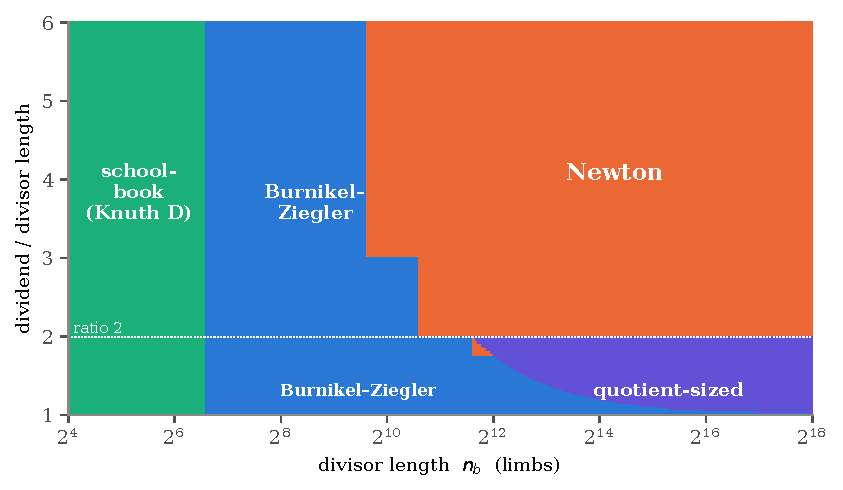
\includegraphics[width=0.88\textwidth]{figures/div_dispatch_map.pdf}
\caption{Which algorithm computes quotient and remainder, by divisor length and length
ratio. Computed from the dispatcher's rules. (Quotient-only calls with ratio below 2 first
shrink the problem to the operands' top limbs, \cref{sec:toplimbs}.)}
\label{fig:divmap}
\end{figure}

\section{The reasoning behind each region}

\paragraph{Divisor under 96 limbs: long division.} Burnikel--Ziegler bottoms out in the same
Algorithm D kernel, so below about 96 limbs the two tie, and the simpler one wins on
overhead. Above it, Burnikel--Ziegler wins at \emph{every} ratio.

\paragraph{Quotient at least as long as the divisor (ratio $\ge 2$).} Here the reciprocal can be
reused across several blocks, so Newton pays off once the divisor is large enough to make
its multiplications NTT-sized: from 1536 limbs, or from 768 limbs when there are at least
three blocks (ratio $\ge 3$) to share the reciprocal's cost. Below that, Burnikel--Ziegler.

\paragraph{Quotient shorter than the divisor (ratio $< 2$).} Now a full reciprocal of the divisor
is wasteful: it is computed to produce a quotient that only the divisor's top limbs
determine. So:
\begin{itemize}
  \item a long quotient ($\ge 3072$ limbs) uses quotient-sized division, Newton on the operands'
        tops plus one back-multiplication;
  \item a large divisor with ratio at least $7/4$ (almost two blocks) still uses Newton;
  \item everything else uses Burnikel--Ziegler, which for a thin quotient already does
        ``divide the tops, multiply back once''.
\end{itemize}

\begin{keyidea}
Long division when the divisor is short; recursive block division in the middle; Newton when
a reciprocal can be reused over several blocks; and when the quotient is short, work only
with the top limbs.
\end{keyidea}

\section{Worked dispatch examples}

\begin{example}[s: which algorithm divides?]
\begin{description}[leftmargin=1.2cm,style=nextline]
  \item[$5000 \div 50$ limbs] Divisor below 96: \textbf{Algorithm D}. Cost about
        $4951 \times 50$ limb steps.
  \item[$2000 \div 1000$] Ratio 2, divisor below 1536, ratio below 3:
        \textbf{Burnikel--Ziegler}.
  \item[$4000 \div 1000$] Ratio 4, divisor $\ge 768$: \textbf{Newton}; one reciprocal shared
        by about three blocks.
  \item[$20\,000 \div 15\,000$, with remainder] $\delta = 5000 \ge 3072$ and smaller than the
        divisor: \textbf{quotient-sized}. Divides the top $\approx 10\,004$ by $5004$ limbs,
        then one $5000 \times 15\,000$ product.
  \item[$10\,500 \div 10\,000$, with remainder] $\delta = 500$, ratio 1.05:
        \textbf{Burnikel--Ziegler}.
  \item[$10\,500 \div 10\,000$, quotient only] $\delta + 4 = 504 < 10\,000$:
        \textbf{top limbs}. Divides the top $1004$ limbs of $a$ by the top $504$ of $b$ (through
        the dispatcher again, which picks Burnikel--Ziegler), and almost never needs the
        confirming product.
  \item[$a \div 7$] One-limb divisor: \textbf{short division}.
\end{description}
\end{example}

\section{How good are the choices?}

The rule was fitted on a grid of divisor lengths from 32 to 262\,144 limbs times
11 ratios from 1.02 to 10, with every algorithm timed directly. Before the re-sweep the
dispatcher was more than 10\% slower than the best algorithm on 69 of 232 grid cells (up to
2.8 times); after it, 3 cells (all under 16\%).

Dispatcher time relative to GMP 6.3, geometric mean over the 11 ratios (single run, M1 Max):

\begin{center}
\small
\begin{tabular}{rcc}
\toprule
divisor limbs & before the 2026-11 re-sweep & after \\
\midrule
32--96 & 1.24--1.27$\times$ & 1.24--1.26$\times$ \\
384 & 1.83$\times$ & 1.35$\times$ \\
768 & 2.19$\times$ & 1.37$\times$ \\
2048 & 1.11$\times$ & 1.08$\times$ \\
4096 & 0.90$\times$ & 0.85$\times$ \\
12288 & 0.61$\times$ & 0.55$\times$ \\
32768 & 0.69$\times$ & 0.61$\times$ \\
\bottomrule
\end{tabular}
\end{center}

Below about 2000 limbs GMP's hand-written assembly is still 1.25--1.4 times faster; from about
4000 limbs BigMath's threaded NTT puts it ahead.

\begin{practice}
\begin{itemize}
  \item Use \code{a / b} when you only need the quotient. For a quotient shorter than the
        divisor it can be dozens of times faster than \code{DivideAndRemainder}, because only the
        top limbs are divided.
  \item Use \code{DivideAndRemainder(a, b)} when you need both: one division gives both, which is
        cheaper than \code{a / b} followed by \code{a \% b}.
  \item Use \code{CachedDivision} when the divisor repeats.
\end{itemize}
\end{practice}
